\documentclass{beamer}


% \usepackage{CJKnumb}\usepackage{beamerthemesplit}

\mode<article>
{
  \usepackage{beamerbasearticle}
  \usepackage{fullpage}
  \usepackage{hyperref}
}

%\usepackage{beamerthemesplit} 
%\usepackage{beamerthemeshadow}  
%\usepackage[width=2cm,dark,tab]{beamerthemesidebar}


% Setup appearance:

%\usetheme{Darmstadt}
\usefonttheme[onlylarge]{structurebold}
\setbeamerfont*{frametitle}{size=\normalsize,series=\bfseries}
\setbeamertemplate{navigation symbols}{}

\renewcommand\arraystretch{1.5}

% Standard packages

\usepackage[english]{babel}
%\usepackage[latin1]{inputenc}

\usepackage{epsf}
\usepackage{amsmath,amssymb}
\usepackage{graphicx}
\usepackage{tabularx}

% \usepackage[usenames,dvipsnames]{color}
\definecolor{shadow}{gray}{0.8}
\newcommand{\redc}[1]{{\color{red} #1}}
\newcommand{\blackc}[1]{{\color{black} #1}}
\newcommand{\bluec}[1]{{\color{blue} #1}}
\newcommand{\shadowc}[1]{{\color{shadow} #1}}
\definecolor{myyellow}{HTML}{FFB700}
\newcommand{\yellowc}[1]{{\color{myyellow} #1}}
\newcommand{\greenc}[1]{{\color{green} #1}}
\newcommand{\whitec}[1]{{\color{white} #1}}
\newcommand{\vect}[1]{\textbf{\textit{#1}}}
\renewcommand{\d}[1]{\textrm{#1}}


\usepackage{amsfonts}
\newcommand{\tickYes}{\checkmark}
\usepackage{pifont}
\newcommand{\tickNo}{\hspace{1pt}\ding{55}}

\usetheme{Boadilla}
% \usetheme{Copenhagen}
% \usetheme{Madrid}
%\usetheme{Singapore}


\begin{document}
%\title{Comparative atomistic and coarse-grained study of water: Simulation details vs. Simulation feasibility}
%\title[Optimizing SPME]{Optimizing Working Parameters of the Smooth Particle Mesh Ewald Algorithm}
\title[Error estimates of Ewald, SPME \& StME]{
  On the numerical accuracy of Ewald, smooth particle mesh Ewald, and staggered mesh Ewald methods for inhomogeneous and correlated molecular systems
}
\author{Han Wang}
\institute[FU-Berlin] {
  Institute for Mathematics, Freie Universit\"at Berlin, Germany
\vskip 0.4cm
Joint with: Christof Sch\"utte (FUB\&ZIB), Pingwen Zhang (PKU)}
\date[Sept. 2013]{09 Sept. 2013\\ACS 246th National Meeting}
\frame{\titlepage}

\begin{frame}{Electrostatic interaction in a periodic boundary system}
  \begin{itemize}
    \vfill
  \item<1-> \bluec{$N$} point charges in the system and we know:\\
    \bluec{$\vect r_1, \vect r_2, \cdots, \vect r_N$}, and
    \bluec{$q_1, q_2, \cdots, q_N$}.
    \vfill
  \item <2-> Periodic boundary condition.
    \vfill
  \item <3-> Coulomb's law, the electrostatic interaction:
    \begin{equation*}\bluec{
        U_{\textrm{ele}} =
        \frac12 \sum^\ast_{\vect n}\sum_{0\leq i,j\leq N}
        \frac{1}{4\pi\epsilon_0\epsilon}\cdot
        \frac{q_i q_j}{\vert \vect r_{ij} + \vect n\vert}}
    \end{equation*}
    \vfill
  \item <4-> Difficulty of treating this sum: Slow convergence.
    \vfill
  \end{itemize}  
\end{frame}

\begin{frame}{Ewald summation}
  \begin{itemize}
  \item <1->
    Ewald summation (1921) splits the
    energy into three parts
    \bluec{
      \begin {align*}
        U_{\textrm{ele}} &=  U_{\textrm{dir}} + U_{\textrm{rec}}+ U_{\textrm{corr}}\\
        U_{\textrm{dir}} & = \frac12 \sum^{\ast}_{\vect n}
        \sum_{i,j = 1}^{N} \frac{q_iq_j\, \redc{\textrm{erfc}(\beta \vert\vect{r}_{ij} + \vect{n}\vert)}}
        {\vert\vect{r}_{ij} + \vect{n}\vert} \\ 
        U_{\textrm{rec}} & = \frac1{2\pi V} \sum_{\vect m \neq 0}
        \frac{\redc{\exp(-\pi^2\vect m^2 / \beta^2)}}{\vect m^2} S(\vect m) S(-\vect m) \\
        U_{\textrm{corr}}& = -\frac\beta{\sqrt \pi} \sum_{i=1}^N q_i^2
      \end {align*}}
  \item<2-> \bluec{$S(\vect m)$} is the structure factor
    defined by \bluec{
      $\sum_{j=1}^N q_j \exp (2 \pi i \vect m \cdot \vect r_j)$.}
  \end{itemize}
\end{frame}


\begin{frame}{Smooth Particle Mesh Ewald Method (SPME)}{An $\mathcal O(N \log N)$ method}
  \begin{itemize}\itemsep -5pt
  \item<1-> Optimal computational complexity of the Ewald summation\footnote{
    \bluec{J. Perram, H. Petersen and S. De Leeuw, Mol. Phys. \textbf{65}, 875 (1988).}}: \redc{$\mathcal O(N^{1.5})$}.
    \vskip .5cm
  \item<2-> \redc{S}mooth \redc{P}article \redc{M}esh \redc{E}wald
    (\redc{SPME})\footnote{
    \bluec{U. Essmann, \textit{et. al.}, J. Chem. Phys. \textbf{103}, 8577 (1995).}}: interpolate \bluec{$S(\vect m)$} on grid, then FFTs on the grid.
    The computational cost is 
  \begin{align*}
    \begin{tabular}[t]{c}
      \redc{$\mathcal O(N)$}\\
      {direct}
    \end{tabular}
    +
    \begin{tabular}[t]{c}
      \redc{$\mathcal O(N)$}\\
      {interpolation}
    \end{tabular}
    +
    \begin{tabular}[t]{c}
      \redc{$\mathcal O(N\log N)$}\\
      {FFTs}
    \end{tabular}
    =
    \begin{tabular}[t]{c}
      \redc{$\mathcal O(N\log N)$}\\
      {total cost}
    \end{tabular}
    \end{align*}
  \item <3-> Two force methods:\\
    \redc{ik-differentiation} and \redc{analytical differentiation}.
  \end{itemize}
\end{frame}

\begin{frame}{Staggered Mesh Ewald (StME) Method}
  \begin{itemize}
  \item <1-> The staggered mesh.
    \begin{figure}
      \centering
      \includegraphics[width=0.4\textwidth]{figs/staggered-mesh/st-mesh.eps}
    \end{figure}
  \item <2->Force scheme:
    \bluec{
      \begin{align*}
        \vect F_{rec}^{st} = \frac12\times (\blackc{\vect F_{rec}^{1}} + \redc{\vect F_{rec}^2})
      \end{align*}
    }
  \end{itemize}
\end{frame}

\begin{frame}{The working parameters of SPME and StME}
  \begin{itemize}
  \vfill
  \item <1->
    SPME parameters:
  \vfill
    \begin{itemize}
    \item \redc{$\beta$} \quad The controlling parameter.
    \item \redc{$r_c$} \quad The direct space cut-off radius.
    \item \redc{$\vect K$} \quad The reciprocal space cut-off. The number of FFT grid points.
    \item \redc{$n$} \quad The order of cardinal B-spline interpolation.
    \end{itemize}
    \vfill
  \item <2->
    An arbitrary combination may lead to \redc{totally wrong results}.
  \item <3->
    \vfill
    Which is the \redc{best combination of parameters}?
  \item <4->
    \vfill
    \redc{Which force method} is better: ik- or ananlytical differentiation?
    \vfill
  \end{itemize}
\end{frame}

\begin{frame}{Why do we need an error estimate as a function of working parameters?}
  \begin{itemize}\itemsep-.5cm
  \item <1-> Define the ``error''
    \bluec{
    \begin{align*}
      \Delta\vect F = \vect F_{real} - \vect F_{calculated},
      \qquad \mathcal E({\beta}, r_c, n, {\vect K}) = \sqrt{\langle\vert \Delta\vect F \vert^2\rangle}
    \end{align*}}
\item<2-> A visulization of
  \bluec{$ \mathcal E =  \mathcal E(\redc{\beta}, r_c, n, \redc{\vect K})$}
    \begin{figure}
    \centering
    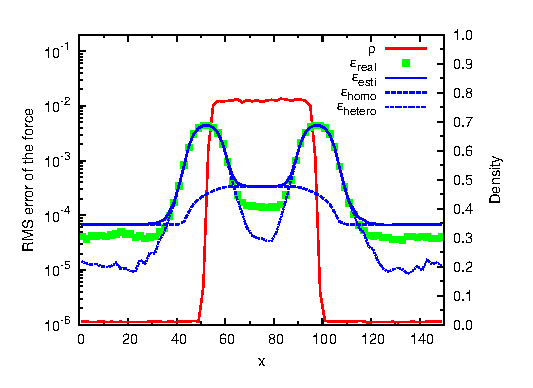
\includegraphics[width=0.7\textwidth]{figs/long-range/error-uniform.eps}
  \end{figure}
  \vfill
  \end{itemize}
\end{frame}

\begin{frame}{The optimal working parameters for SPME \& StME}
  \begin{itemize}
  \item <1-> The computational expense:
    \bluec{
      \begin{align*}
        \mathcal T ({\beta}, r_c, n, {\vect K})
        \propto
        \mathcal O(r_c^3) +
        \mathcal O(n^3) +
        \mathcal O(K_1K_2K_3\log(K_1K_2K_3))
      \end{align*}
    }
  \item <2->The optimization problem:
    \bluec{
      \begin{align*}
        \min & \quad\mathcal T\,({\beta}, r_c, n, {\vect K}),\\
        \textbf{s.t.} &
        \quad \mathcal E\,({\beta}, r_c, n, {\vect K}) \leq
        \mathcal E_{\textrm{control}}
      \end{align*}
    }
    An effective numerical solotion to this problem is in Ref.~\footnote{
    \bluec{H. Wang, F. Dommert and C. Holm, J. Chem. Phys. \textbf{133}, 034117 (2010).}}
  \end{itemize}
\end{frame}

\begin{frame}{Existing results and limitations}
  \begin{itemize}
    \vfill
  \item <1-> Ewald summation \& SPME (\tickYes).  StME (?)\\
    \vfill
  \item <2-> Limitations:
    \redc{1. Homogeneous},
    \redc{2. Uncorrelated}
    \vfill
  \item <3-> A realistic system...
    \vskip -.2cm
    \begin{figure}
      \centering
      \includegraphics[width=0.9\textwidth]{figs/sys-confs/inhomo-corr-1.pdf}
      \hfill
    \end{figure}
    \vfill
  \end{itemize}
\end{frame}

\begin{frame}{The error estimate for inhomogeneous and correlated systems}
  \begin{itemize}
  \item <1-> Define the error force kernel
    \bluec{
      \begin{align*}
        \Delta \vect F(\vect r)
        &=
        q \sum_{j=1}^N q_j \,\vect K(\vect r, \vect r_j)
      \end{align*}}
  \item <2->
    Example: If the interaction is calculated by the cut-off method:
    \bluec{
      \begin{align*}
        \vect F_{ij} =
        \left\{
          \begin{array}{ll}
            \vect f(\vert\vect r_i-\vect r_j\vert), & \vert\vect r_i - \vect r_j\vert\leq r_c; \\
            0, & \vert\vect r_i - \vect r_j\vert > r_c.
          \end{array}
        \right.      
    \end{align*}
    }
    The kernel is:
    \bluec{
      \begin{align*}
        \vect K(\vect r_i,\vect r_j) =
        \left\{
          \begin{array}{ll}
            0, & \vert\vect r_i - \vect r_j\vert\leq r_c; \\
            \vect f(\vert\vect r_i-\vect r_j\vert), & \vert\vect r_i - \vect r_j\vert > r_c.
          \end{array}
        \right.
      \end{align*}}
    \vfill
  \end{itemize}
\end{frame}

\begin{frame}{The error estimate for inhomogeneous and correlated systems}
  \begin{itemize}\itemsep -10pt
  \item<1->   The mean error force is
    \bluec{
      \begin{align*}
        \langle\Delta\vect F(\vect r)\rangle
        =
        q\int_{\mathbb R^3}\vect K(\vect r , \vect r')\,\rho_q(\vect r')\,\d d\vect r'
      \end{align*}
    }
  \vskip -10cm
\item<2->   The error:
  \bluec{
    \begin{align*} \nonumber
      % \langle\vert\Delta\vect F(\vect r)\vert^2\rangle
      \mathcal E^2
      = 
      \redc{\mathcal E^2_{\textrm{homo}}(\vect r)} +
      % \langle\Delta\vect F(\vect r)\,\rangle^2 +
      \redc{\mathcal E^2_{\textrm{inhomo}}(\vect r)} +
      \redc{\mathcal E_{\textrm{correlation}}(\vect r)}.
    \end{align*}
  }
  with\bluec{
  \begin{align*}
    \redc{\mathcal E^2_{\textrm{homo}}(\vect r)}
    = &\,
    q^2\int_{\mathbb R^3}\vert\vect K(\vect r, \vect r')\vert^2\rho_{q^2}(\vect r')\,\d d\vect r'  \\
    \redc{\mathcal E^2_{\textrm{inhomo}}(\vect r)}
    = &\,
    q^2\bigg[\int_{\mathbb R^3}\vect K(\vect r, \vect r')\rho_q(\vect r')\,\d d\vect r'\,\bigg]^2
    \\
    \redc{\mathcal E_{\textrm{correlation}}(\vect r)}
    =&\,
    q^2\int_{\mathbb R^3\times\mathbb R^3}\vect K(\vect r, \vect r')\cdot\vect K(\vect r, \vect r'')\,C_{q^2}(\vect r', \vect r'')\,\d d\vect r'\d d\vect r''
  \end{align*}}
  \end{itemize}
\end{frame}

\begin{frame}{The error estimate for inhomogeneous and correlated systems}
  \begin{itemize}
  \item <1-> The mean error force:
    \bluec{
      \begin{align*}
        \langle\Delta\vect F(\vect r)\rangle
        =&\,
        q\int_{\mathbb R^3}\vect K(\vect r , \vect r')\,\rho_q(\vect r')\,\d d\vect r'     \\
        \rho_{q}(\vect r) =&\,
        \langle \sum_{j=1}^Nq_j\,\delta(\vect r - \vect r_j) \rangle        
      \end{align*}}
  \item <2-> The inhomogeneity error:
    \bluec{
      \begin{align*}
        {\mathcal E^2_{\textrm{inhomo}}(\vect r)}
        &=
        q^2\bigg[\int_{\mathbb R^3}\vect K(\vect r, \vect r')\rho_q(\vect r')\,\d d\vect r'\,\bigg]^2\\
        & 
        \redc{ = \langle\Delta\vect F(\vect r)\,\rangle^2}
      \end{align*}}
    \bluec{$\rho_{q}(\vect r)$} vanishes when the system is \redc{locally neutral}.
  \end{itemize}
\end{frame}


\begin{frame}{The error estimate for inhomogeneous and correlated systems}
  \begin{itemize}
  \item <1-> The homogeneity error:
    \bluec{
      \begin{align*}
        {\mathcal E^2_{\textrm{homo}}(\vect r)}
        = &\,
        q^2\int_{\mathbb R^3}\vert\vect K(\vect r, \vect r')\vert^2\rho_{q^2}(\vect r')\,\d d\vect r'  \\
        \rho_{q^2}(\vect r) =&\,
        \langle \sum_{j=1}^Nq^2_j\,\delta(\vect r - \vect r_j) \rangle
      \end{align*}}    
  \item <2-> The correlation error:
    \bluec{
      \begin{align*}
        \mathcal E_{\textrm{correlation}}(\vect r)
        =&\,
        q^2\int_{\mathbb R^3\times\mathbb R^3}\vect K(\vect r, \vect r')\cdot\vect K(\vect r, \vect r'')\,C_{q^2}(\vect r', \vect r'')\,\d d\vect r'\d d\vect r''
      \end{align*}
      \blackc{with}
      \begin{align*}
        C (\vect r, \vect r') =&\,
        \rho^{(2)}(\vect r, \vect r') -
        \rho_{q}(\vect r)\rho_{q}(\vect r') \\
        \rho^{(2)}(\vect r, \vect r') =&\,
        \langle \sum_{i\neq j}^Nq_jq_j\,\delta(\vect r - \vect r_i)\,\delta(\vect r - \vect r_j) \rangle
      \end{align*}
    }
  \end{itemize}
\end{frame}


\begin{frame}{Two findings concerning StME}
  \begin{itemize}
    \vfill
  \item <1-> StME is always more precise than SPME.
    \vfill
  \item <2-> The ik- and ananlytical differentiation are equivalent for StME.
    \vfill
  \end{itemize}
\end{frame}


\begin{frame}{Computational feasiability}
  \begin{itemize}
    \vfill
  \item <1->
    If the error kernel has
    \bluec{
      \begin{align*}
        \vect K(\vect r, \vect r') = \vect K(\vect r - \vect r')
      \end{align*}
    }
  \item <2-> Ewald and StME.
    \vfill
  \item <3-> SPME under approximations.
    \vfill
  \item <4-> Every term is convolution:
    \begin{align*}
      \begin{tabular}[t]{c}
      \bluec{$\mathcal E^2$}\\
      {}
    \end{tabular}
    =
    \begin{tabular}[t]{c}
      \bluec{$q^2[\vect K^2\ast \rho_{q^2}]$}\\
      \bluec{$\mathcal O(N\log N)$}
    \end{tabular}
    +
    \begin{tabular}[t]{c}
      \bluec{$q^2[\vect K\ast \rho_q]^2$}\\
      \bluec{$\mathcal O(N\log N)$}
    \end{tabular}
    +
    \begin{tabular}[t]{c}
      \bluec{$q^2 \vect K\ast[\vect K\ast C]$}\\
      \bluec{$\mathcal O(N^\redc{2}\log N)$}
    \end{tabular}
    \end{align*}
    \vfill
  \end{itemize}
\end{frame}
  % \item <3->
  %   Nearest neighbor approx.:
  %   \bluec{$\mathcal O(N^\redc{2}\log N)\longrightarrow \mathcal O(N\log N)$} 
  %   \vfill


\begin{frame}{Numerical check: the inhomogeneity error}
  \begin{figure}
    \centering
    \includegraphics[width=0.8\textwidth]{figs/long-range-inhomo/rand1-rho.eps}
  \end{figure}
\end{frame}

\begin{frame}{Numerical check: the inhomogeneity error}
  \begin{figure}
    \centering
    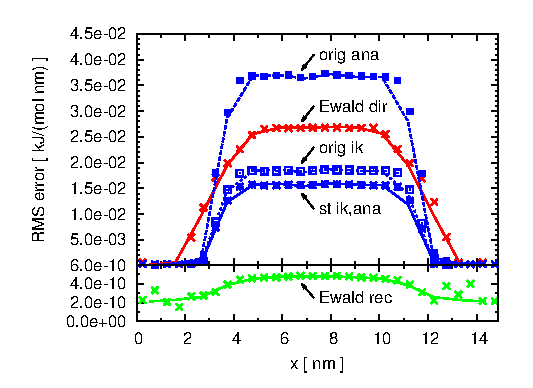
\includegraphics[width=0.8\textwidth]{figs/long-range-inhomo/rand1-error.eps}
  \end{figure}
\end{frame}

\begin{frame}{Numerical check: the inhomogeneity error}
  \begin{figure}
    \centering
    \includegraphics[width=0.8\textwidth]{figs/long-range-inhomo/rand2-rho.eps}
  \end{figure}
\end{frame}

\begin{frame}{Numerical check: the inhomogeneity error}
  \begin{figure}
    \centering
    \includegraphics[width=0.8\textwidth]{figs/long-range-inhomo/rand2-error.eps}
  \end{figure}
\end{frame}

\begin{frame}{Real inhomogeneity water system: bad news}{StME method real error v.s. estimated error}
  \begin{figure}
    \centering
    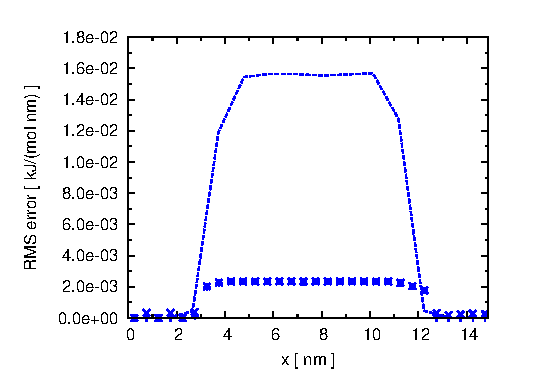
\includegraphics[width=0.8\textwidth]{figs/long-range-inhomo/water-st-error-1.eps}
  \end{figure}  
\end{frame}

\begin{frame}{Bond correlation}
  \begin{figure}
    \centering
    \includegraphics[width=0.8\textwidth]{figs/long-range-inhomo/correlation.pdf}
  \end{figure}    
\end{frame}


\begin{frame}{The nearest neighbor approximation of the correlation error}
  \begin{itemize}
  \item <1-> The correlation function is approximated:
    \bluec{
      \begin{align*}
        C(\vect r, \vect r') \approx
        \big\langle \sum_j\sum_{k\in\redc{\Omega_j}} q_jq_k
        \delta (\vect r' - \vect r_j)\delta (\vect r' - \vect r_k)\big\rangle
      \end{align*}
    }
    $\redc{\Omega_j}$: the nearest neighbors of \bluec{$j$}.
    \vfill
  \item <2-> The bonded correlation:
    \bluec{\begin{align*}
        \mathcal E_{\textrm{correlation}}(\vect r) &=
        q^2 [(\vect K\cdot (\hat T_O\hat{\vect K})^\vee) \ast \rho_O]+
        q^2 [(\vect K\cdot (\hat T_H\hat{\vect K})^\vee) \ast \rho_H] \\
        \hat T_O(\vect m) &= 2 \langle q_He^{-2\pi i\vect m\cdot s_O}\rangle\\
        \hat T_H(\vect m) &=
        \langle q_O e^{-2\pi i\vect m\cdot s_O} +
        q_H e^{-2\pi i\vect m\cdot s_H}\rangle
      \end{align*}}
    \bluec{$T_O(\vect m)$}  and  \bluec{$T_O(\vect m)$}  intrinsic structure.
    \vfill
  \item <3-> Computational cost:
    \bluec{$\mathcal O(N^\redc{2}\log N)\longrightarrow \mathcal O(N\log N)$}
  \end{itemize}
\end{frame}

\begin{frame}{Nearest neighbor approximation of the correlation error}{Bonded correlation}
  \begin{figure}
    \centering
    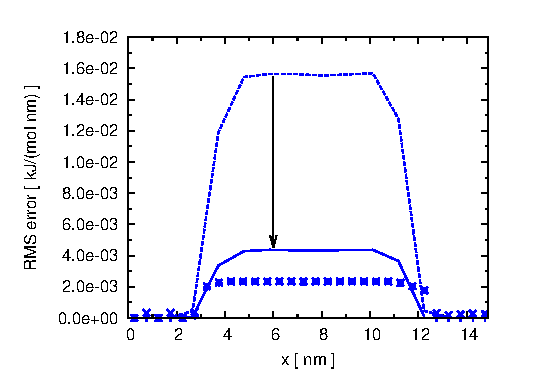
\includegraphics[width=0.8\textwidth]{figs/long-range-inhomo/water-st-error-2.eps}
  \end{figure}  
\end{frame}

\begin{frame}{Nonbonded near neigbor correlation}{radial distribution functions}
  \begin{itemize}
  \item <1-> Nonbonded correlation: radial distribution functions (RDFs).
    \bluec{
    \begin{align*}
          \hat T_{\textrm{O}} (\vect m)
    &= \int_0^{\redc{R_g}}
    [q_{_{\textrm{H}}} \rho_{_{\textrm{H}}} \tilde g_{_{\textrm{OH}}}(r)
    +q_{_{\textrm{O}}} \rho_{_{\textrm{O}}} \tilde g_{_{\textrm{OO}}}(r)]
    \,\frac{\sin(2\pi m r)}{2\pi mr}\,4\pi r^2 \d dr,\\\label{eqn:nb-nna-2}
    \hat T_{\textrm{H}} (\vect m)
    &= \int_0^{\redc{R_g}}
    [q_{_{\textrm{H}}} \rho_{_{\textrm{H}}} \tilde g_{_{\textrm{HH}}}(r)
    +q_{_{\textrm{O}}} \rho_{_{\textrm{O}}} \tilde g_{_{\textrm{OH}}}(r)]
    \,\frac{\sin(2\pi m r)}{2\pi mr}\,4\pi r^2 \d dr,
  \end{align*}
  }
  \item <2-> Convergence w.r.t. \redc{$R_g$}
    \begin{figure}
    \centering
    \raisebox{0.08\height}{\includegraphics[width=0.42\textwidth]{figs/long-range-nna/rdf-corr-1.eps}}
    \hfill
    \includegraphics[width=0.46\textwidth]{figs/long-range-nna/fig-gr.eps}
  \end{figure}
  \end{itemize}
\end{frame}


\begin{frame}{Nearest neighbor approximation of the correlation error}{Bonded \& nonbonded correlation}
  \begin{figure}
    \centering
    \includegraphics[width=0.8\textwidth]{figs/long-range-inhomo/water-st-error-3.eps}
  \end{figure}  
\end{frame}

\begin{frame}{In a wider  range of parameters}
  \begin{figure}
    \centering
    \includegraphics[]{figs/long-range-nna/fig-order-st.eps}
  \end{figure}  
\end{frame}

\begin{frame}{In a wider range of parameters}
  \begin{figure}
    \centering
    \includegraphics[]{figs/long-range-nna/fig-mesh-st.eps}
  \end{figure}  
\end{frame}

\begin{frame}{\whitec{Thanks}}
  \begin{figure}
    \centering
    \raisebox{1.5pt}{\includegraphics[]{figs/long-range-nna/fig-mesh-st-1.eps}}
  \end{figure}  
\end{frame}







\end{document}
